\documentclass[draft]{article}
\usepackage{cmap}
\usepackage[T1,T2A]{fontenc}
\usepackage[utf8]{inputenc}
\usepackage[russian]{babel}
\usepackage[left=2cm,right=2cm,top=2cm,bottom=2cm,bindingoffset=0cm]{geometry}
\usepackage{tikz}


\usepackage{setspace,amsmath}
\usepackage{lipsum}
\usepackage[usestackEOL]{stackengine}
\usepackage{kantlipsum}
\usepackage{graphicx}
\usepackage{caption}
\usepackage{float}
\usetikzlibrary{positioning}
\graphicspath{{pictures/}}
\DeclareGraphicsExtensions{.pdf,.png,.jpg}
\newcommand\zz[1]{\par{\normalsize\strut #1} \hfill\ignorespaces}
\addto\captionsrussian{\def\refname{List of used sources}}
\newcommand{\subtitle}[1]{%
  \posttitle{%
    \par\end{center}
    \begin{center}\Large#1\end{center}
   }%
}
\newcommand{\subsubtitle}[1]{%
  \preauthor{%
    \begin{center}
    \large #1 \vskip0.5em
    \begin{tabular}[t]{c}
    }%
}
\newcommand\tab[1][1cm]{\hspace*{#1}}
\begin{document}
 
\begin{center}
\textbf{
ПРАВИТЕЛЬСТВО РОССИЙСКОЙ ФЕДЕРАЦИИ\\
НАЦИОНАЛЬНЫЙ ИССЛЕДОВАТЕЛЬСКИЙ УНИВЕРСИТЕТ\\
«ВЫСШАЯ ШКОЛА ЭКОНОМИКИ»\\
Факультет компьютерных наук
Образовательная программа «Программная инженерия»\\
(ВШЭ ФКН ПИ)}\\
\end{center}
УДК 004.852
\bigskip
\zz{Руководитель,}Выполнил:
\zz{Стажер-исследователь,}Студент группы БПИ204
\zz{приглашённый лектор}образовательной программы
\zz{\noindent\rule{3cm}{0.4pt} О. Н. Качан}«Программная инженерия»
\zz{«\noindent\rule{1cm}{0.4pt}»\noindent\rule{2cm}{0.4pt}20\noindent\rule{0.5cm}{0.4pt}г.}Пеганов Никита Сергеевич
\zz{~}\noindent\rule{3cm}{0.4pt}Н.С. Пеганов
\zz{~}«\noindent\rule{1cm}{0.4pt}»\noindent\rule{2cm}{0.4pt}20\noindent\rule{0.5cm}{0.4pt}г.
\begin{center}
\topskip=0pt
\vspace*{\fill}
\textbf{ОТЧЕТ\\
О НАУЧНО-ИССЛЕДОВАТЕЛЬСКОЙ РАБОТЕ}\\
~\\
SYNCHRONIZATION OF NEUROMORPHIC NETWORKS OF THE SMALL WORLD IN KURAMOTO MODEL\\
(заключительный)\\
\vspace*{\fill}
\end{center}
\begin{center}
\vspace*{\fill}{
  Москва 2022}
\end{center}
\newpage
\begin{center}
\section {Abstract}
\end{center}
\tab Neurons in our brains are connected by a network of connections called synapses. Synapses are the sites where neurons communicate with each other, and they are important for learning and memory.\\
~\\
\tab Understanding how neurons and synapses function to make up the brain is essential to understanding how they work in the rest of the body. Understanding how the brain works will help us to understand how to treat problems like Alzheimer’s disease and other neurological disorders.\\
~\\
\tab If we consider the brain as a graph we will see that all neurons are divided into groups. This groups are connected with each other with a small number of synapses. But they are tightly connected within these groups. The type of communication of neurons within a group is called "small world graph".\\
~\\
\tab We can define a small world network as a network in which there is not a strong connection between any two nodes, but there are many connections between each node and the rest of the network. In a small world system there are no paths of length greater than four that connect all the nodes of the system.\\
~\\
\tab This is the reason why the graph of the close world model is chosen in this paper. In this case, the number of links between any two nodes is very small.\\
~\\
\tab The object of research of this work is the synchronization of neurons. The goal is to understand the mechanisms that underlie the generation of synchronized activity in large populations of neurons, and to identify the functional roles of each mechanism. In particular, the goal is to develop a better understanding of the relationships between the properties of neuronal networks and their behavior under physiological conditions. This will be accomplished by studying the effects of changing the network's characteristics on its behavior.\\
~\\
\newpage
\begin{center}
\section {Content}
\tableofcontents
\end{center}
\newpage
\section {Basic terms, definitions and abbreviations}
\tab \textbf{Graph} — a set of items connected by edges. A graph G can be defined as a pair (V,E), where V is a set of vertices, and E is a set of edges between the vertices  $E \subseteq \{(u,v) | u, v \in V\}$\cite{litlink1}.\\
~\\
\tab \textbf{Simplicial complex} $K$ (sometimes called an abstract simplicial complex) consists of
\begin{enumerate} 
\item a set of objects, V(K), called vertices
\item a set, $S(K)$, of finite non-empty subsets of $V(K)$, called simplices.
\end{enumerate}
such that the simplices satisfy the following conditions:
\begin{enumerate} 
\item if $\sigma\subset V(K)$ is a simplex and $\tau\subset\sigma, \tau\neq\emptyset$, then $\tau$ is also a simplex;
\item every singleton {v}, $v\in V(K)$, is a simplex\cite{litlink4}.
\end{enumerate}			
A graph is \textbf{globally synchronized} if in the long-run all oscillators are in phase, starting from all initial conditions except a set of measure zero\cite{litlink8}.\\
~\\
\tab \textbf{Synchronization} — the fact of happening at the same time, or the act of making things happen at the same time\cite{litlink2}.\\
~\\
\tab \textbf{Simplicial synchronization} — a fundamental dynamical state observed in a wide variety of complex systems and capturing among other phenomena important aspects of brain dynamics and circadian rhythms\cite{litlink3}.\\
~\\
\tab \textbf{Kuramoto model} is a stylized model that explains how coupled oscillators, that in absence of interactions would have different intrinsic frequencies, can start to follow a collective coherent motion when their coupling constant $\sigma$, measuring the strength of their interaction, is larger than a critical value $\sigma_c$ also called synchronization threshold\cite{litlink3}.\\

\newpage
\begin{center}
\item\section {Introduction}
\end{center}
\textbf{Task description}\\
\tab Analysis of the small-world graphs' syncing by Kuramoto model. That means checking how the neuron network will synchronize after deleting one of it's neurons.
~\\
\textbf{Relevance}\\
\tab Neurons in our brain are placed as small-world graph. So, understanding of the ways of their synchronization will help us to get closer to understanding the work of the brain, as well as to find new methods of treating brain diseases. This theme is actual nowadays which shows a large number of recent works.\\
~\\
\textbf{Subject of research}\\
\tab The subject of the research is small-world graphs' synchronization. Small-world networks are characterized by their fast adaptation to external perturbations, yet are not able to respond quickly to internal changes. We use these properties in order to study the possibility of synchronization of a random small-world network.\\
~\\
\textbf{Research methods}\\
\tab The way of research is reading of scientific literature on a related topic and analysis of the information. Also there is an experement that checks the hypothesis.\\
~\\
\textbf{Purposes and objectives of the work}\\
\tab The purpose of the research is checking the hypothesis of neurons synchronization in small-world graphs.\\
The objectives of the work are:\\
\begin{enumerate} 
\item to find the information on the selected topic in the works of other researchers
\item analyze and aggregate fount information
\item select and describe used methods and algorithms
\item conduct an experiment to check the hypothesis
\item analyze the results of the experiment
\item draw conclusions
\end{enumerate} 
~\\
\textbf{Originality and reliability of the obtained results}\\
\tab During the analysis of sources, it was found out that there are works on related topics, but it is not sufficiently studied.\\
~\\
\textbf{Theoretical significance}\\
\tab The work has a theoretical significance as a research of a significant process for medicine — neuron syncing. The way to calculate the level of synchronization is universally used Kuramoto model. So, the work can be used in other researchs.\\
~\\
\textbf{Practical value}\\
\tab Neuromorphic computing is not very practically used method because artificial methods of machine learning are better in most tasks. But the code (you can find it in Application 1) can be used in some brain simulation tasks.\\
~\\
\newpage
\begin{center}
\section {The main part of the research report}
\end{center}
\begin{center}
\textbf{Review and analysis of sources}\\
\end{center}
\tab\textbf{"Geometry, Topology and Simplicial Synchronization"\cite{litlink3}} by Ana Paula Millán, Juan G. Restrepo, Joaquín J. Torres and Ginestra Bianconi is a review article fully covering the area under study. It defines "Simplicial synchronization", "Kuramoto model", "Graph Laplacian" and other important definitions. \\
\tab In this article Ginestra Bianconi explores how the combinatorial and statistical properties of complex networks have effects on dynamics. Simplical complexes affect on higher-order dynamics through simplical geometry and topology. To research it two frameworks are used: Network Geometry with Flavor (NGF) and Graph Laplacian. Exactly, spectral dimension of NGF networks is used to measure the gemetry influence on dynamics.\\
\tab The level of synchronization in the system is measured by the
Kuramoto order parameter,
\begin{center}
$Z_0 = R_0e^{i\Theta} = \frac{1}{N} \sum_{j=1}^{N_[0]}e^{i\theta _j}$,
\end{center}
where $R_0$ and $\Theta$ are both real and where $0<=R_0<=1$ measures the overall coherence and $\Theta = \Theta (t)$ is the phase of global oscillations.
\tab As the result of the research we have several formulas that can determine the level of syncronization of complexes with differtent geometry and topology.
\begin{figure}[h]
\center{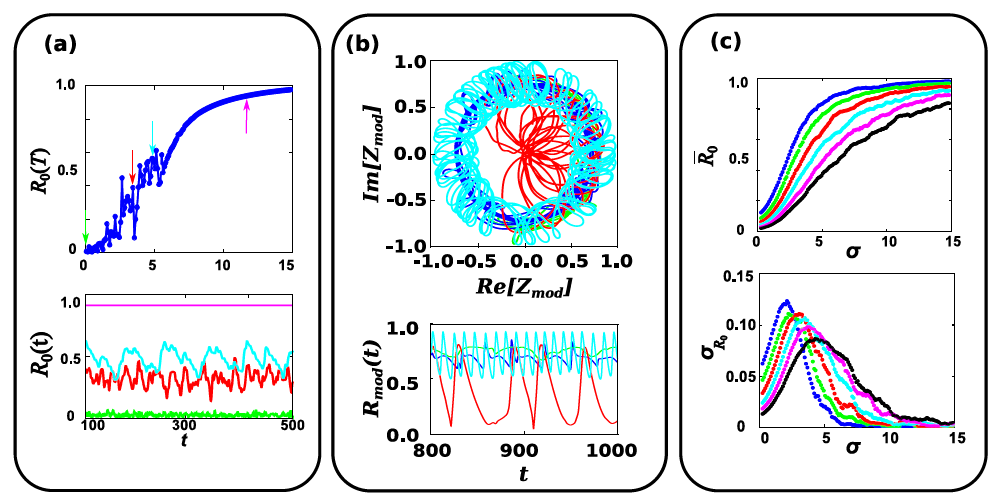
\includegraphics[draft=false,width=1\linewidth]{Fig1}}
\caption{Frustrated synchronization on NGF characterized by spatio-temporal fluctuations of the order parameter\cite{litlink3}.}
\label{ris:image}
\end{figure}\\
\tab \textbf{"Higher-order simplicial synchronization of coupled topological signals"\cite{litlink5}} by Reza Ghorbanchian, Juan G. Restrepo, Joaquin J. Torresy, and Ginestra Bianconi shows the possible phase transitions that can occur when topological signals dened on nodes and links interact. This research is based on the mathematical framework of higher-order topological synchronization. For some reasons, in this work authours focus in particular on the coupled synchronization of topological signals dened on nodes and links.\\
\tab Interestingly, in this research more mathematical frameworks has been chosen: models NL and NLT, Geometry with Flavor (NGF) and Kuramoto model for measuring the level of synchronization in the system.\\
\tab This work uncovers how topological signals associated to nodes and links can be coupled to one another giving rise to an explosive synchronization phenomenon involving both signals at the same time. Created model has been tested on real connectomes and on major examples of simplicial complexes (the conguration model of simplicial complex and the Network Geometry with Flavor).\\
~\\
\begin{figure}[h]
\center{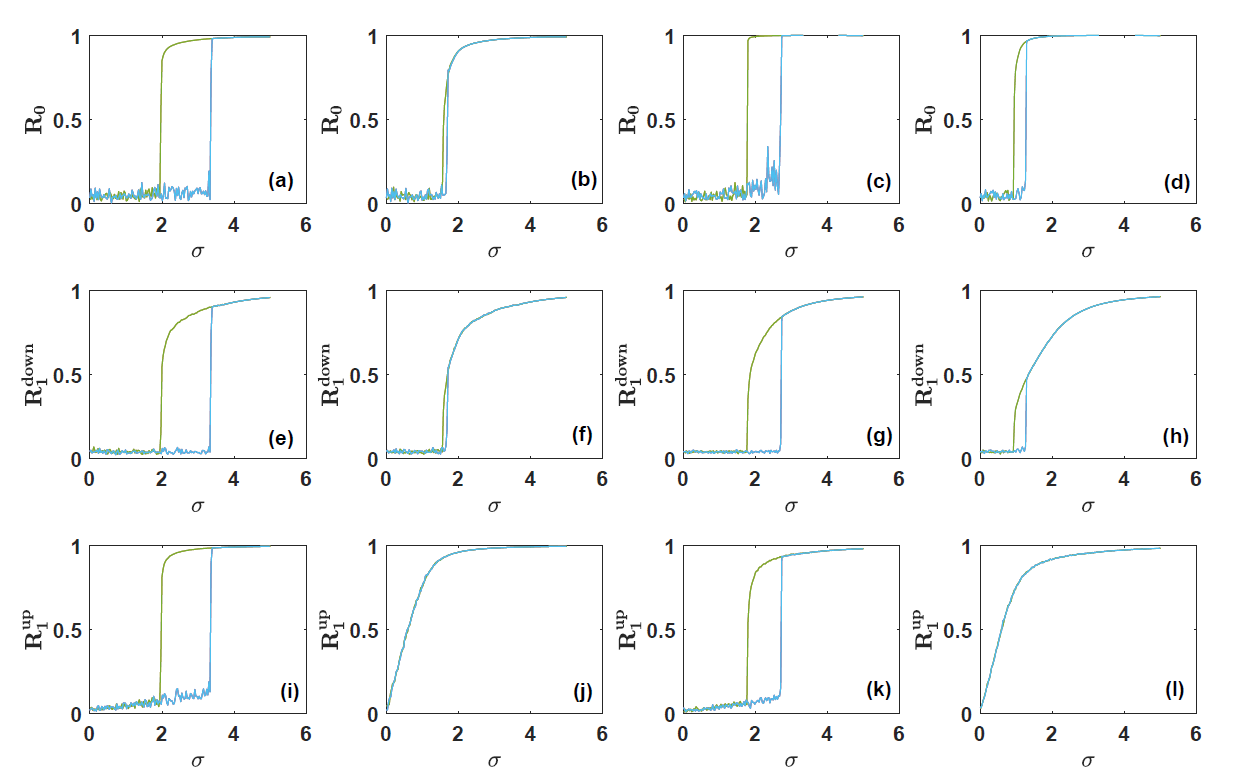
\includegraphics[draft=false,width=1\linewidth]{Fig2}}
\caption{The Higher-order topological synchronization models (Models NL and NLT) coupling nodes and links on simplicial complexes\cite{litlink6}.}
\label{ris:image}
\end{figure}\\
~\\
\tab In work \textbf{"Explosive higher-order Kuramoto dynamics on simplicial complexes"} Ana P. Millán, Joaquín J. Torres, Ginestra Bianconi show, how complexes behave on higher-order interactions.\\
\tab In this work the configuration model Configuration of simplicial complexes is used, which naturally generalizes the configuration model of networks. There are also exist Farber, Emergent, Hyperbolic and Petri-dynamical models.\\
\tab So, authors show, that higher-order Kuramoto dynamics are defined on faces of dimension $n-1$ and $n+1$, which follow a dynamics of coupled oscillators. This work opens innovative perspectives in characterizing the Kuramoto dynamics on higher dimensional simplices.\\
\begin{figure}[h]
\center{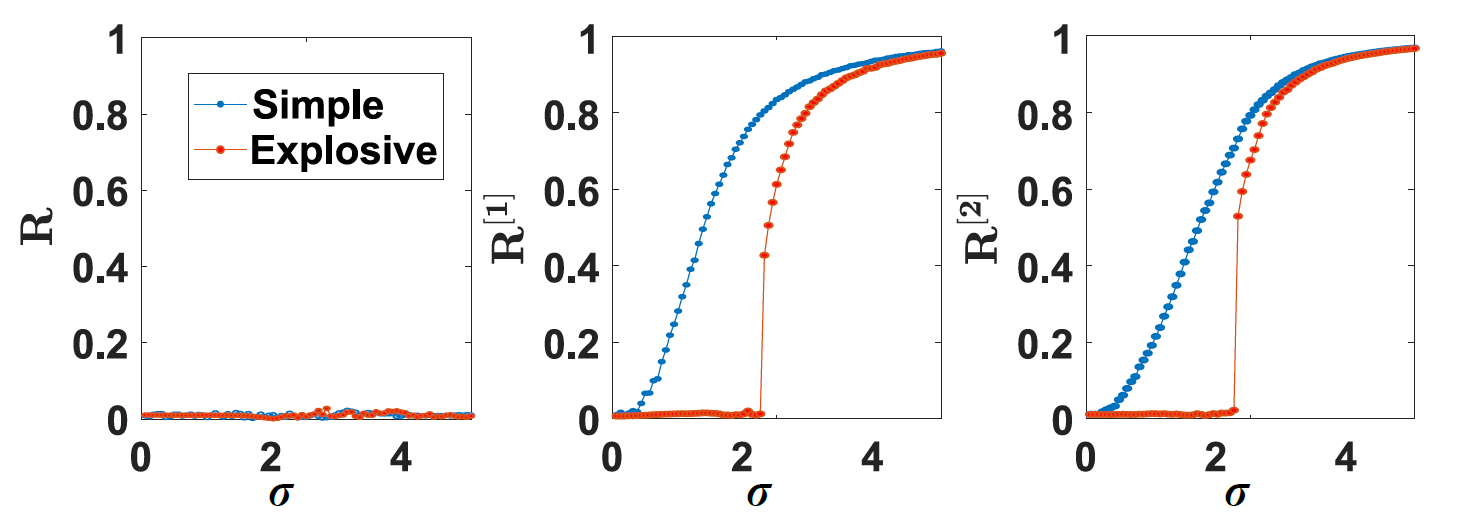
\includegraphics[draft=false,width=1\linewidth/2]{Fig3}}
\caption{The order parameters R, R[1] and R[2] of the simple (blue circles) and explosive (red squares) higher-order $(n = 1)$. Kuramoto dynamics are plotted versus the coupling constant $\sigma$.\cite{litlink7}.}
\label{ris:image}
\end{figure}\\
\begin{center}
\textbf{Selection of methods, algorithms, models for solving tasks}\\
\end{center}
\tab As mentioned above, the type of graph is small-world. This type of graphs was chosen because of the similarity with the structure of the human brain. The human brain is a very complex organ and it is difficult to find the exact structure of its network. However, it has been shown that the neuronal networks of the brain possess the properties of small-world networks.\\
~\\
\tab Neuromorphic computing is a form of computing that has recently received a lot of attention due to the fact that it is based on the natural brain. Neuromorphic computers are based on biological neurons and synapses. And this is the way to most fully simulate the human brain. The term “neuromorphic” refers to an artificial neural network that mimics the function of a biological neural network.\\
~\\
\tab To assess the level of synchronization of neurons, the Kuramoto model was chosen. This model is a mathematical framework to describe the dynamics of a network of interacting oscillators. The Kuramoto model has been widely used in the study of brain dynamics. A Kuramoto oscillator is defined as a system of coupled phase oscillators, where each oscillator has a fixed frequency and the phase of each oscillator varies around the average phase of the entire population, so that the sum of all phases is zero.\\
~\\
\tab Another way to evaluate the synchronization of neurons is to calculate their total activity. This is done by summing the number of spikes that each neuron produces during a given time interval. The mean number of spikes per neuron during the time window is then computed. An example of such a plot is shown in Figure 4.\\
\begin{figure}[h]
\center{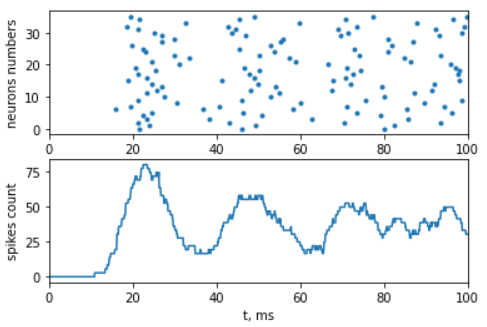
\includegraphics[draft=false,width=1\linewidth/2]{Fig4}}
\caption{Graph of the total activity of neurons of the small world network.}
\label{ris:image}
\end{figure}\\
\begin{center}
\textbf{Description of selected or proposed methods, algorithms, models, techniques}\\
\end{center}
\tab For the convenience of development, the python language was chosen. The Python is a programming language that enables you to write programs in a simple way. It has a syntax that is easy to learn and that allows you to easily add new features. For example, the Python language allows you to do a lot of things with graphs, such as adding nodes and edges, creating and manipulating graphs.\\
~\\
\tab The Networkx library is used to create the small-world graph. NetworkX is a Python package for the creation, manipulation, and study of the structure, dynamics, and functions of complex networks.\\
~\\
\tab The brian2 library was used to stimulate the work of neurons. It is an experimental simulation environment that can be used for testing and debugging of neural network models and hardware implementations. This allows the development of a wide variety of neural model architectures for the generation of different kinds of signals.\\
~\\
\tab Finally, the kuramoto library\cite{litlink9} is used to calculate the level of synchronization of neurons according to the Kuramoto model. This library allows you to calculate the synchronization level and also draw a plot of all the time series and oscillators in complex plane at different times.\\
\begin{center}
\textbf{Description of the experiment}\\
\end{center}
\tab At first, random small-world graph has been generated. It's side is 6 and the count of vertexes is 36. These numbers have been selected in case of the best time of syncing. Synchronization also occurs on other sources, but these numbers were chosen for the presentation as the most suitable.
\begin{figure}[h]
\center{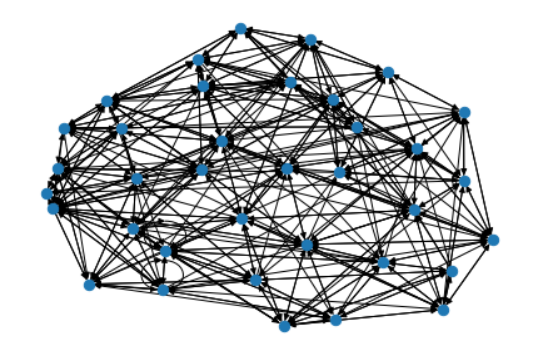
\includegraphics[draft=false,width=0.5\linewidth]{Fig5}}
\caption{Example small-world graph.}
\label{ris:image}
\end{figure}\\
~\\
\tab Thereafter, a neural network based on this model was compiled. The method of the neuron group generation is Euler method. The output of the model is the plot of spikes of the neurons and their counts.
\begin{figure}[h]
\center{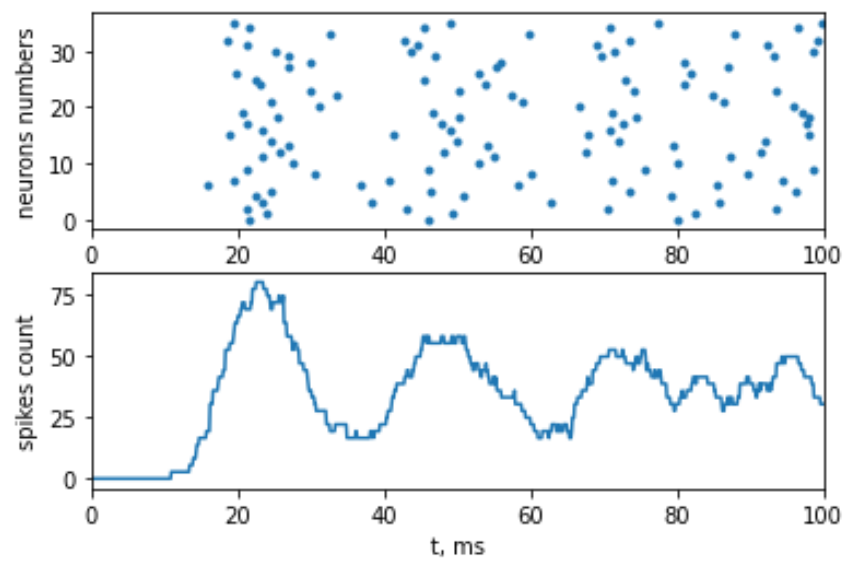
\includegraphics[draft=false,width=0.5\linewidth]{Fig6}}
\caption{The graph of neurons syncing.}
\label{ris:image}
\end{figure}\\
~\\
\tab Also let's calculate the phase by Kuramoto model. In the Kuramoto oscillator, the phase of each node is defined as the angle between node's position vector and the average position of all nodes.
\begin{figure}[h]
\center{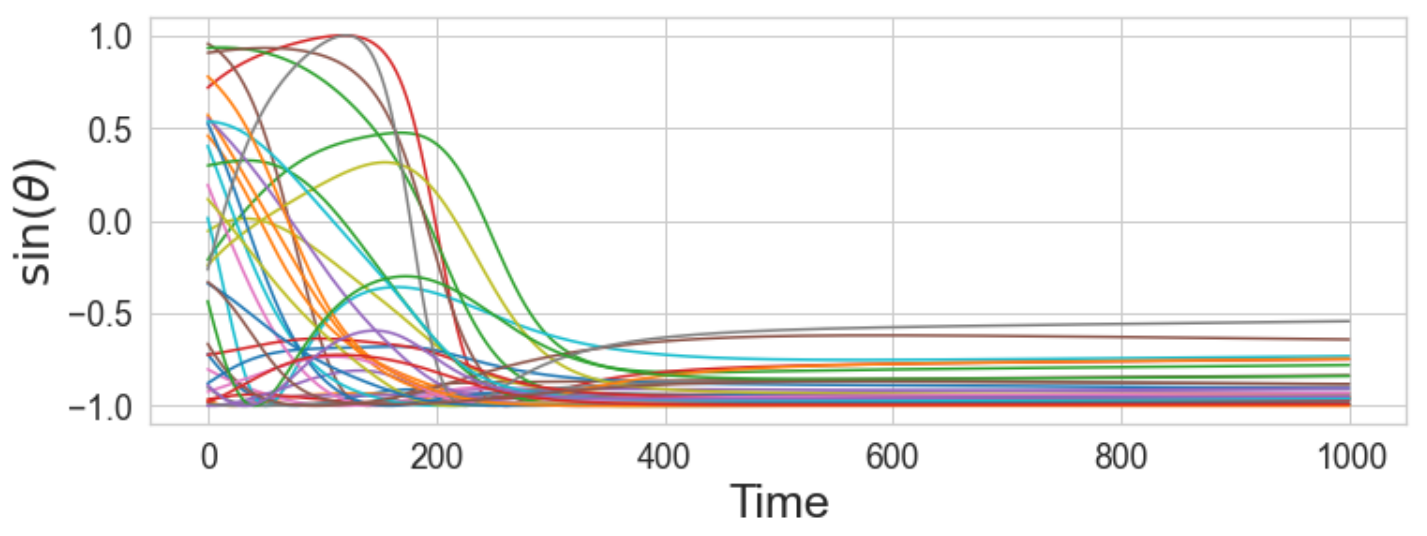
\includegraphics[draft=false,width=0.5\linewidth]{Fig7}}
\caption{The phase of every oscillator for all the time series.}
\label{ris:image}
\end{figure}\\
\tab We can see that both characteristics show synchronization's success.\\
~\\
\newpage
\tab Then we should delete one neuron to check new level of synchronization. For this propose, all it's synapses have been simply deleted.
\begin{figure}[h]
\center{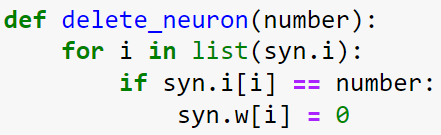
\includegraphics[draft=false,width=0.5\linewidth]{Fig8}}
\caption{The code of neuron deletion.}
\label{ris:image}
\end{figure}\\
\tab Then start the net processing again and check it's syncing by both metrics.
\begin{figure}[h]
\center{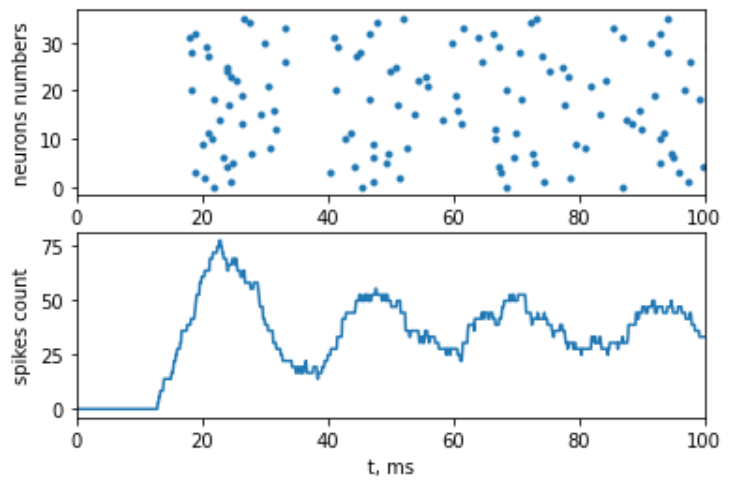
\includegraphics[draft=false,width=0.5\linewidth]{Fig9}}
\caption{The plot of total neurons activity after deleting one of them.}
\label{ris:image}
\end{figure}\\
\begin{figure}[h]
\center{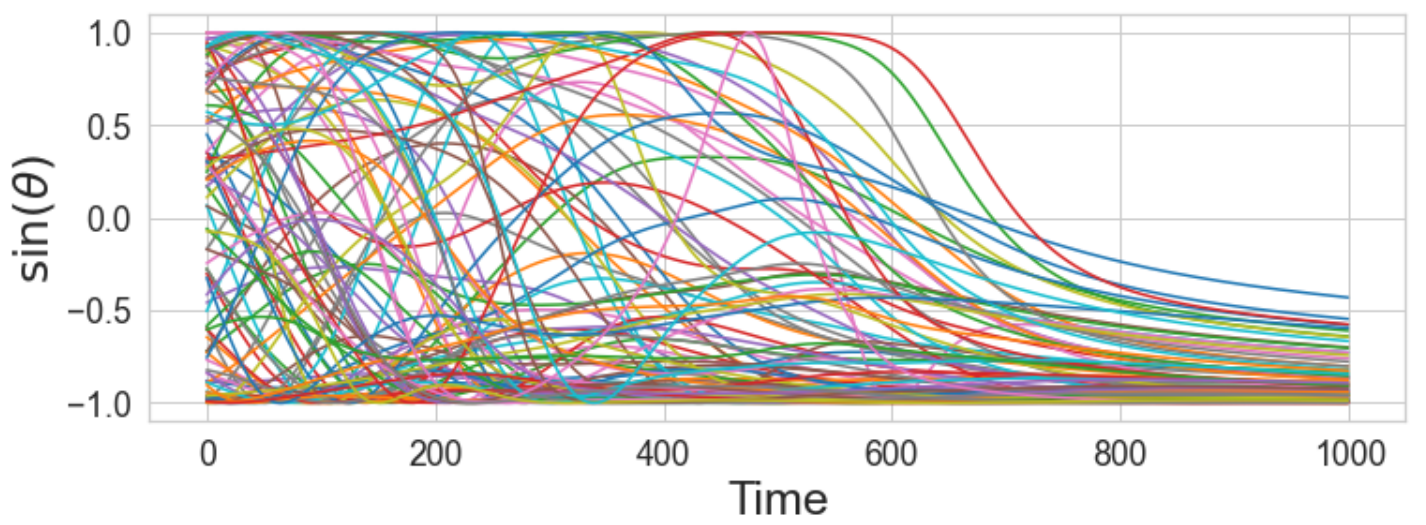
\includegraphics[draft=false,width=0.5\linewidth]{Fig10}}
\caption{The plot of neurons activity after deleting one of them in Kuramoto model.}
\label{ris:image}
\end{figure}\\
\newpage
\begin{center}
\section {Conclusion}
\end{center}
\tab In this paper, an analysis of the literature was carried out. Simplicial complex, Kuramoto model and other important definitions were found. The application of these models in the theory of neuromorphic systems is also described.\\
~\\
\tab The methods and algorithms used in the study are selected and described. The model of graph is small-world model due to it's similarity with brain's structure. Neuromorphic computing is a way to simulate the neuronet working. And Kuramoto model is the method of synchronization's measurement.\\
~\\
\tab The plot of neurons' activity has been built two times: before and after deleting one of the neurons. They show that synchronization time increases after deleting but the synchronization does not disappear. So, the hypothesis is confirmed: neuron deleting does not affect on network syncing.\\
\newpage
\begin{center}
\begin{thebibliography}{}
\bibitem{litlink1} \textit{Paul E. Black and Paul J. Tanenbaum} "graph", in Dictionary of Algorithms and Data Structures [online], Paul E. Black, ed. 21 June 2021. (accessed 04.07.2022) Available from: https://www.nist.gov/dads/HTML/graph.html
\bibitem{litlink2} \textit{Cambridge University Press} Meaning of synchronization in English. // Website dictionary.cambridge.org (https://dictionary.cambridge.org/dictionary/english/synchronization). Viewed: 04.07.2022
\bibitem{litlink3} \textit{Ana Paula Millán, Juan G. Restrepo, Joaquín J. Torres and Ginestra Bianconi} Geometry, Topology and Simplicial Synchronization. P. 12
\bibitem{litlink4} Simplicial complex. // Website ncatlab.org (https://ncatlab.org/nlab/show/simplicial+complex). Viewed: 09.07.2022
\bibitem{litlink5} \textit{Reza Ghorbanchian, Juan G. Restrepo, Joaquin J. Torresy, and Ginestra Bianconi} Higher-order simplicial synchronization of coupled topological signals. // Website Arxiv.org (https://arxiv.org/abs/2011.00897). Viewed: 11.07.2022
\bibitem{litlink6} \textit{Reza Ghorbanchian, Juan G. Restrepo, Joaquin J. Torresy, and Ginestra Bianconi} Higher-order simplicial synchronization of coupled topological signals. P. 6
\bibitem{litlink7} \textit{Ana P. Millan, Joaquin J. Torres,  Ginestra Bianconi} Explosive higher-order Kuramoto dynamics on simplicial complexes. // Website Arxiv.org (https://arxiv.org/abs/1912.04405). Viewed: 11.07.2022
\bibitem{litlink8} \textit{Alex Townsend, Michael Stillman, Steven H. Strogatz} Dense networks that do not synchronize and sparse ones that do. // Website Arxiv.org (https://arxiv.org/abs/1906.10627). Viewed: 01.09.2022
\bibitem{litlink9} \textit{fabridamicelli} Python implementation of the Kuramoto model. // Website Github.com (https://github.com/fabridamicelli/kuramoto). Viewed: 04.09.2022
\end{thebibliography}
\end{center}
\newpage
\begin{center}
\section {Applications}
\end{center}
\zz{}\textbf{Application 1\\}
Link to the project repository with the source code and all used materials.\\
https://github.com/NikPeg/synchronization-of-neuromorphic-networks-of-the-close-world-from-the-point-of-view-of-complexes\\
\end{document}